\title{Linear Mixed Effects Models}

\subsection{Linear Mixed Effects Models}

With linear mixed effects models, we wish to model a linear
relationship for data points with inputs of varying type, categorized
into subgroups, and associated to a continuous output.

We demonstrate with an example in Edward.
An interactive version with Jupyter notebook is available
\href{http://nbviewer.jupyter.org/github/blei-lab/edward/blob/master/docs/notebooks/linear_mixed_effects_models.ipynb}{here}.

\subsubsection{Data}

We use the \texttt{InstEval} data set from the popular
\href{http://lme4.r-forge.r-project.org}{lme4 R package}
\citep{bates2015fitting}, located
\href{https://github.com/blei-lab/edward/blob/master/examples/data/insteval.csv}{here}.
It is a data set of instructor evaluation ratings, where the inputs
(covariates) include categories such as \texttt{students} and
\texttt{departments}, and our response variable of interest is the
instructor evaluation rating.

\begin{lstlisting}[language=Python]
data = pd.read_csv('../../examples/data/insteval.csv')
data['dcodes'] = data['d'].astype('category').cat.codes
data['deptcodes'] = data['dept'].astype('category').cat.codes
data['s'] = data['s'] - 1

train = data.sample(frac=0.8)
test = data.drop(train.index)
\end{lstlisting}

In the code, we denote:
\begin{itemize}
\item \texttt{students} as \texttt{s}
\item \texttt{instructors} as \texttt{d}
\item \texttt{departments} as \texttt{dept}
\item \texttt{service} as \texttt{service}
\end{itemize}

\begin{lstlisting}[language=Python]
n_s = 2972  # number of students
n_d = 1128  # number of instructors
n_dept = 14  # number of departments
n_obs = train.shape[0]  # number of observations
\end{lstlisting}

\subsubsection{Model}

With linear regression, one makes an independence assumption among data
points. In our setting, the observations come from sets of
groups which may have varying slopes and intercepts. Thus we'd like to
build a model that can capture this behavior \citep{gelman2006data}.

For example:
\begin{itemize}
\item The observations from a single student are not independent of
each other. Rather, some students may systematically give low (or
high) lecture ratings.
\item The observations from a single teacher are not independent of
each other. We expect good teachers to get generally good ratings and
bad teachers to get generally bad ratings.
\item The observations from a single department are not independent of
each other. One department may generally have dry material and thus be
rated lower than others.
\end{itemize}

Typical linear regression takes the form
\begin{equation*}
\mathbf{y} = \mathbf{X}\beta + \epsilon,
\end{equation*}
where $\mathbf{X}$ corresponds to fixed effects with coefficients
$\beta$ and $\epsilon$ corresponds to random noise,
$\epsilon\sim\mathcal{N}(\mathbf{0}, \mathbf{I})$.

In a linear mixed effects model, we add an additional term
$\mathbf{Z}\eta$, where $\mathbf{Z}$ corresponds to random effects
with coefficients $\eta$. The model takes the form
\begin{align*}
\eta &\sim \mathcal{N}(\mathbf{0}, \sigma^2 \mathbf{I}), \\
\mathbf{y} &= \mathbf{X}\beta + \mathbf{Z}\eta + \epsilon.
\end{align*}
Our goal is to infer $\beta$, $\eta$, and $\sigma^2$, where $\beta$
are model parameters (``fixed effects''), $\eta$ are latent
variables (``random effects''), and $\sigma^2$ is variance component
parameter.

Because the random effects have mean 0, the data's mean is captured by
$\mathbf{X}\beta$, and $\mathbf{Z}\eta$ captures variation (e.g.
Instructor \#54 is rated 1.4 points higher than the mean).

A natural question is the difference between fixed and random effects.
A fixed effect is an effect that is constant for a given population. A
random effect is an effect that varies for a given population (i.e.,
it may be constant within subpopulations but varies within the overall
population). We illustrate below in our example:

\begin{itemize}
\item
Let the fixed effects be for \texttt{service}, which is a binary
covariate corresponding to whether the lecture belongs to the
lecturer's main department or not. No matter how much additional data
we collect, it can only take on the values in $0$ and $1$.
\item
Let the random effects be for the categorical values of
\texttt{students}, \texttt{teachers}, and \texttt{departments}. Given
more data, we may be looking at new students, teachers, or
departments.
\end{itemize}

In summary, given covariates \texttt{students}, \texttt{teachers},
\texttt{departments}, and \texttt{service}, we aim to analyze the
instructor's evaluation ratings. In the syntax of R's lme4 package
\citep{bates2015fitting}, this can be written as

\begin{lstlisting}[language=JSON]
y ~ 1 + (1|students) + (1|instructor) + (1|dept) + service
\end{lstlisting}
where \texttt{(1|x)} denotes that \texttt{x} is a random effect and not
fixed.

\begin{lstlisting}[language=Python]
# Set up placeholders for the data inputs.
s_ph = tf.placeholder(tf.int32, [None])
d_ph = tf.placeholder(tf.int32, [None])
dept_ph = tf.placeholder(tf.int32, [None])
service_ph = tf.placeholder(tf.float32, [None])

# Set up fixed effects.
mu = tf.Variable(tf.random_normal([]))
service = tf.Variable(tf.random_normal([]))

sigma_s = tf.sqrt(tf.exp(tf.Variable(tf.random_normal([]))))
sigma_d = tf.sqrt(tf.exp(tf.Variable(tf.random_normal([]))))
sigma_dept = tf.sqrt(tf.exp(tf.Variable(tf.random_normal([]))))

# Set up random effects.
eta_s = Normal(mu=tf.zeros(n_s), sigma=sigma_s * tf.ones(n_s))
eta_d = Normal(mu=tf.zeros(n_d), sigma=sigma_d * tf.ones(n_d))
eta_dept = Normal(mu=tf.zeros(n_dept), sigma=sigma_dept * tf.ones(n_dept))

yhat = tf.gather(eta_s, s_ph) + \
    tf.gather(eta_d, d_ph) + \
    tf.gather(eta_dept, dept_ph) + \
    mu + service * service_ph
y = Normal(mu=yhat, sigma=tf.ones(n_obs))
\end{lstlisting}

\subsubsection{Inference}

Given data, we aim to infer the random effects of each category as
well as estimates of the model's fixed effects.

In this analysis, we use variational inference with the
$\text{KL}(q\|p)$ divergence measure. We specify fully factorized
normal approximations for the random effects and pass in all training
data for inference. Under the algorithm, the fixed effects will be
optimized in a variational EM scheme.

\begin{lstlisting}[language=Python]
q_eta_s = Normal(
    mu=tf.Variable(tf.random_normal([n_s])),
    sigma=tf.nn.softplus(tf.Variable(tf.random_normal([n_s]))))
q_eta_d = Normal(
    mu=tf.Variable(tf.random_normal([n_d])),
    sigma=tf.nn.softplus(tf.Variable(tf.random_normal([n_d]))))
q_eta_dept = Normal(
    mu=tf.Variable(tf.random_normal([n_dept])),
    sigma=tf.nn.softplus(tf.Variable(tf.random_normal([n_dept]))))

latent_vars = {
    eta_s: q_eta_s,
    eta_d: q_eta_d,
    eta_dept: q_eta_dept}
data = {
    y: y_train,
    s_ph: s_train,
    d_ph: d_train,
    dept_ph: dept_train,
    service_ph: service_train}
inference = ed.KLqp(latent_vars, data)
\end{lstlisting}

One way to critique our inferred model is a residual plot, i.e., a
plot of the difference between the predicted value and the observed
value for each data point. Below we manually run inference,
initializing the algorithm and performing individual updates within a
loop. We form residual plots as the algorithm progresses. This helps
us examine how the algorithm proceeds to infer the random and fixed
effects from data.

To form residuals, we first make predictions on test data. We do this
by copying \texttt{yhat} defined in the model and replacing its
dependence on random effects with their inferred means. During the
algorithm, we evaluate the predictions, feeding in test inputs.

\begin{lstlisting}[language=Python]
yhat_test = ed.copy(yhat, {
    eta_s: q_eta_s.mean(),
    eta_d: q_eta_d.mean(),
    eta_dept: q_eta_dept.mean()})
\end{lstlisting}

We now write the main loop.

\begin{lstlisting}[language=Python]
inference.initialize(n_print=20, n_iter=100)
tf.global_variables_initializer().run()

for _ in range(inference.n_iter):
  # Update and print progress of algorithm.
  info_dict = inference.update()
  inference.print_progress(info_dict)

  t = info_dict['t']
  if t == 1 or t % inference.n_print == 0:
    # Make predictions on test data.
    yhat_vals = yhat_test.eval(feed_dict={
        s_ph: s_test,
        d_ph: d_test,
        dept_ph: dept_test,
        service_ph: service_test})

    # Form residual plot.
    plt.title("Residuals for Predicted Ratings on Test Set")
    plt.xlim(-4, 4)
    plt.ylim(0, 800)
    plt.hist(yhat_vals - y_test, 75)
    plt.show()
\end{lstlisting}

\subsubsection{Criticism}

Above, we described a method for diagnosing the fit of the model via
residual plots.
Below we show the residuals for the model post-convergence. (For
intermediate residual plots, check the Jupyter notebook.)

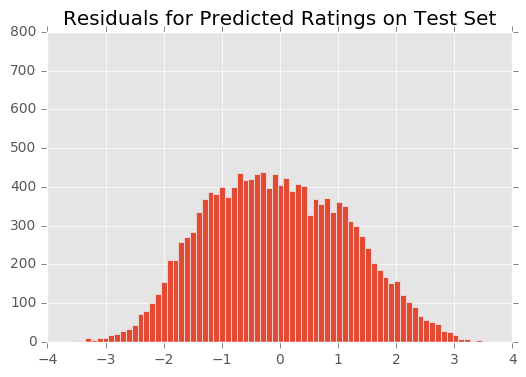
\includegraphics[width=450px]{/images/linear-mixed-effects-models.png}

The residuals appear normally distributed with mean 0. This provides
evidence that the model correctly fits the data.

\subsubsection{Acknowledgments}

We thank Mayank Agrawal for writing the initial version of this
tutorial.

\subsubsection{References}\label{references}
